\chapter{Digráficas de intervalos ajustadas}
\label{cap:DigrafIntAj}

En el año 1989 se publicó un articulo de M. Sen, S. Das, A.B. Roy y D.B. West en el  \textit{Journal of Graph Theory}. En este se introduce una nueva definición que generaliza a las gráficas de intervalos. Dicha generalización iba enfocada a tener caracterizaciones análogas a las de las gráficas de intervalos, una de ellas, la propiedad de los unos consecutivos para columnas de la matriz asociada a la gráfica de clanes maximales. 
Desafortunadamente esta definición, no cuenta con un alguna caracterización en términos de estructuras prohibidas, como sí las tienen las gráficas de intervalos, en términos de las tripletas asteroidales y $k$-ciclos sin cuerdas, $k \geq 4$. Así, al solo contar con una caracterización sencilla, a saber, a través de la propiedad de los unos consecutivos, el único algoritmo de reconocimiento para esta clase no es eficiente.

En el artículo arriba mencionado, se define un digráfica de intervalos como una digráfica $G$ la cual admite una representación de pares de intervalos, es decir, para cada vértice $v \in V(G)$, existen $I_v,J_v$ un par de intervalos, y $uv\in E(G)$ si y solo si $I_u$ intersecta a $J_v$. 

En el ánimo de explorar las propiedades de las digráficas de intervalos surge una pregunta muy natural. ¿Puede una digráfica, cuya gráfica subyacente no sea una gráfica de intervalos, ser una digráfica de intervalos? La respuesta puede responderse inmediatamente mediante este primer ejemplo. Comencemos con una digráfica muy sencilla, la cual se muestra en \cref{fig:Dgrf01} y consta únicamente de dos vértices, $v_1, v_2$, y que carece de flechas, así como de lazos. Una representación por pares de intervalos se muestra en la parte inferior, y es fácil comprobar que las incidencias se respetan, pues los cuatro intervalos son ajenos dos a dos. Pero en particular $I_1$ no intersecta a $J_1$ ni a $J_2$ e $I_2$ tampoco intersecta a $J_1$ o a $J_2$. Para responder la pregunta, hacemos la siguiente nota, en la definición de las gráficas de intervalos es implícito que las gráficas cuenten con lazos, mas aún que sean reflexivas. Como primer contraste, en el caso dirigido se pierde esto, como se mostró en el presente ejemplo. Así que el hecho de que la gráfica suyacente no sea gráfica de intervalos no nos arroja mayor información. 

\begin{figure}[H]
  \centering
  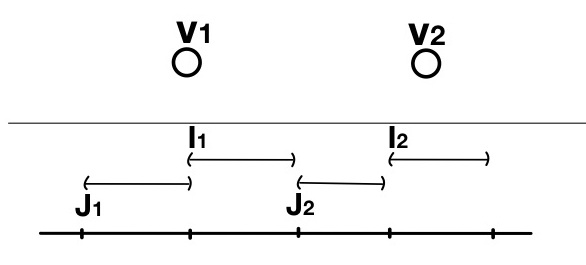
\includegraphics[width=0.5\textwidth]{recursos/capturas/Digraf1.jpg}
  \caption{Digráfica sin flechas ni lazos.}
  \label{fig:Dgrf01}
\end{figure}


Ahora vemos que al añadir una flecha que sale de $v_1$ a $v_2$ nosotros seguimos teniendo que esta digráfica tiene una representación por pares de intervalos. Para dar la representación, podemos usar como base la que se dio en la imagen anterior y solo modificar los intervalos $I_1,J_2$; debemos buscar que $I_1\cap J_2 \neq \emptyset$, es decir, que tengan intersección no vacía, ya que queremos rescatar el hecho de tener la flecha $(v_1,v_2)$. Para lograr esto, basta extender un poco hacia la derecha el extremo derecho del intervalo $I_1$. 

\begin{figure}[H]
  \centering
  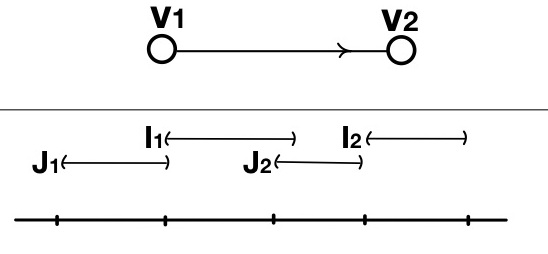
\includegraphics[width=0.5\textwidth]{recursos/capturas/Digraf2.jpg}
  \caption{Digráfica con una sola flecha.}
  \label{fig:Dgrf02}
\end{figure}


A continuación en \cref{fig:Dgrf03} se muestra que al añadir la flecha en el otro sentido se sigue teniendo una representación de pares de intervalos y por tanto se tiene que nuevamente es digráfica de intervalos. Para verificar esto, comenzamos haciendo una pequeña modificación a la representación de pares de la figura anterior. En primer lugar situamos el intervalo $I_2$ a la izquierda de todos los intervalos y extendemos el extremo derecho del intervalo de tal forma que este intersecte al intervalo $J_1$.

\begin{figure}[H]
  \centering
  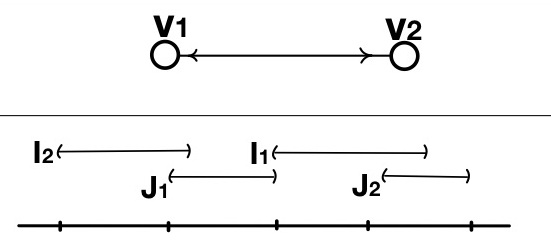
\includegraphics[width=0.5\textwidth]{recursos/capturas/Digraf3.jpg}
  \caption{Digráfica con dos flechas.}
  \label{fig:Dgrf03}
\end{figure}

Finalmente exhibimos que al añadir todas las posibles flechas y lazos en el ejemplo dado en \cref{fig:Dgrf01} seguimos teniendo una digráfica de intervalos. Tomamos la representación del ejemplo anterior y para añadir el lazo en $v_1$ tenemos que $I_1$ debe intersecar a $J_1$ y análogamente tenemos que hacer que $I_2$ intersecte a $J_2$ para así tener el lazo en $v_2$. Notese que $I_1$ e $I_2$ pueden o no intersectarse pues esto no afecta a las flechas, aquí los ponemos disjuntos.

\begin{figure}[H]
  \centering
  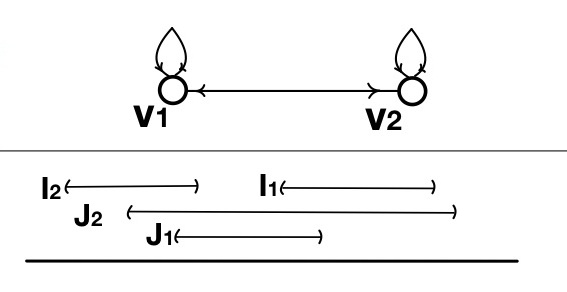
\includegraphics[width=0.5\textwidth]{recursos/capturas/Digraf4.jpg}
  \caption{Digráfica de dos vértices y todas las flechas y lazos posibles.}
  \label{fig:Dgrf04}
\end{figure}
 
Como se vio desde nuestro primer ejemplo, una digráfica de intervalos puede tener como subgráfica subyacente una gráfica la cual no sea de intervalos, como el siguiente ejemplo, el cual tiene como gráfica subyancete un 4-ciclo el cual se vio que no es gráfica de intervalos. 

Ante la ausencia de una caracterización en términos de estrucutras prohibidas sencillas de las digráficas de intervalos, Tomás Feder, Pavol Hell, Jing Huang y Arash Rafiey, publicaron un artículo en 2011 donde introducen una pequeña modificación a las digráficas de intervalos, dando pie a la definición de digráfica de intervalos ajustada. Una digráfica de intervalos ajustada $G$ es una digráfica de intervalos $G$ la cual tiene una representación por pares de intervalos $I_v, J_v$ para cada $v\in V(G)$ de tal forma que $I_v$ y $J_v$ tienen el mismo extremo izquierdo. 

Con este pequeño ajuste, uno vuelve a recuperar la parte de la reflexividad, ya que $I_v,J_v$ tienen el mismo extremo izquierdo, entonces son no ajenos, luego se debe tener que $(v,v)\in E(G)$.

Ahora exploremos unos ejemplos, claramente \crefrange{fig:Dgrf01}{fig:Dgrf03} no pueden ser digráficas de intervalos ajustadas, ya que son no reflexivas. Entonces veamos si al ponerles todos los lazos estas cumplen ser digráficas de intervalos ajustadas.

En el primer caso al añadir los lazos, se tiene la representación de pares de intervalos, cuyos pares de intervalos correspondientes a $v$ tienen el mismo extremo izquierdo. Por tanto, este constituye nuestro primer ejemplo de digráfica de intervalos ajustada.

\begin{figure}[H]
  \centering
  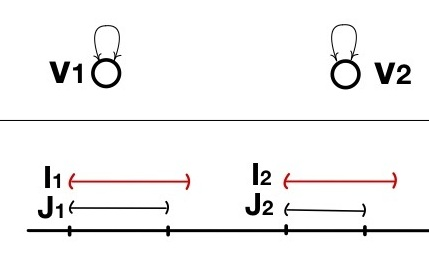
\includegraphics[width=0.4\textwidth]{recursos/capturas/Dgrf_Int_Adj01.jpg}
  \caption{Digráfica de intervalos ajustada. Dos vértices y sin flechas salvo lazos.}
  \label{fig:DgrfAdj01}
\end{figure}

En el segundo ejemplo, se puede encontrar nuevamente una representación por pares de intervalos que satisfaga el ajuste planteado por Tomás Feder et al. 

\begin{figure}[H]
  \centering
  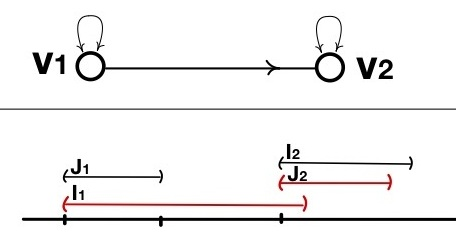
\includegraphics[width=0.45\textwidth]{recursos/capturas/Dgrf_Int_Adj02.jpg}
  \caption{Digráfica de intervalos ajustada. Dos vértices, una flecha.}
  \label{fig:DgrfAdj02}
\end{figure}

Finalmente, si agregamos la flecha $(v_2, v_1)$ entonces damos la siguiente representación ajustada por pares de intervalos. 

\begin{figure}[H]
  \centering
  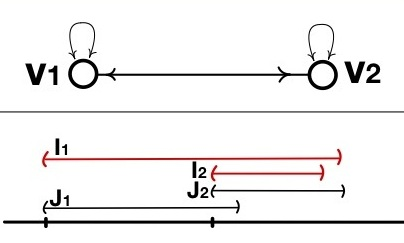
\includegraphics[width=0.45\textwidth]{recursos/capturas/Dgrf_Int_Adj03.jpg}
  \caption{Digráfica de intervalos ajustada con dos vértices y dos flechas.}
  \label{fig:DgrfAdj03}
\end{figure}

A continuación introducimos definiciones muy sencillas. Dado un camino $P=x_0,\dots,x_n$ en una digráfica $G$ y $u,v \in V(G)$ tales que constituyan una flecha, es decir $(u,v) \in E(G)$ o $(v,u) \in E(G)$ decimos que  $(u,v)$ es una flecha derecha si $(u,v) \in E(G)$ y decimos que es una flecha al revés si $(v,u) \in E(G)$. En \cref{fig:DgrfAdj02} podemos decir entonces que $(v_1,v_2)$ es una flecha derecha porque precisamente $(v_1,v_2) \in E(G)$. De forma similar, $(v_2,v_1)$ es una flecha al revés. Sin embargo, uno ve \cref{fig:DgrfAdj03} y se pregunta qué pasa respecto a $(v_1,v_2)$, a estas flechas las cuales sean tanto derechas como al revés, las llamaremos flechas dobles. Aquellas flechas que no son dobles, como la que se muestra en \cref{fig:DgrfAdj02}, se pueden llamar flechas únicamente derechas o únicamente al revés, según sea el caso. Naturalmente los lazos al ser flechas derechas y al revés, son flechas dobles. Si $(u,v)\in E(G)$ diremos que $u$ domina a $v$ o que $v$ es dominado por $u$, sin importar si $(u,v)$ es una flecha doble o única. Esto llevado nuevamente a \cref{fig:DgrfAdj02}, podemos decir entonces que $v_1$ domina a $v_2$. Estas definiciones nos permiten introducir el concepto de caminos congruentes. Dos caminos $P=x_0, \dots, x_n$ y $Q=y_0, \dots, y_n$ en $G$ se dice que son congruentes si tienen el mismo patrón de flechas derechas y al revés, esto es $P,Q$ son caminos congruentes si y solo si $( x_i,x_{i+1})$ es flecha derecha si y solo si $(y_i, y_{i+1})$ es flecha derecha, para toda $0\leq i \leq n-1 $.

\begin{figure}[H]
  \centering
  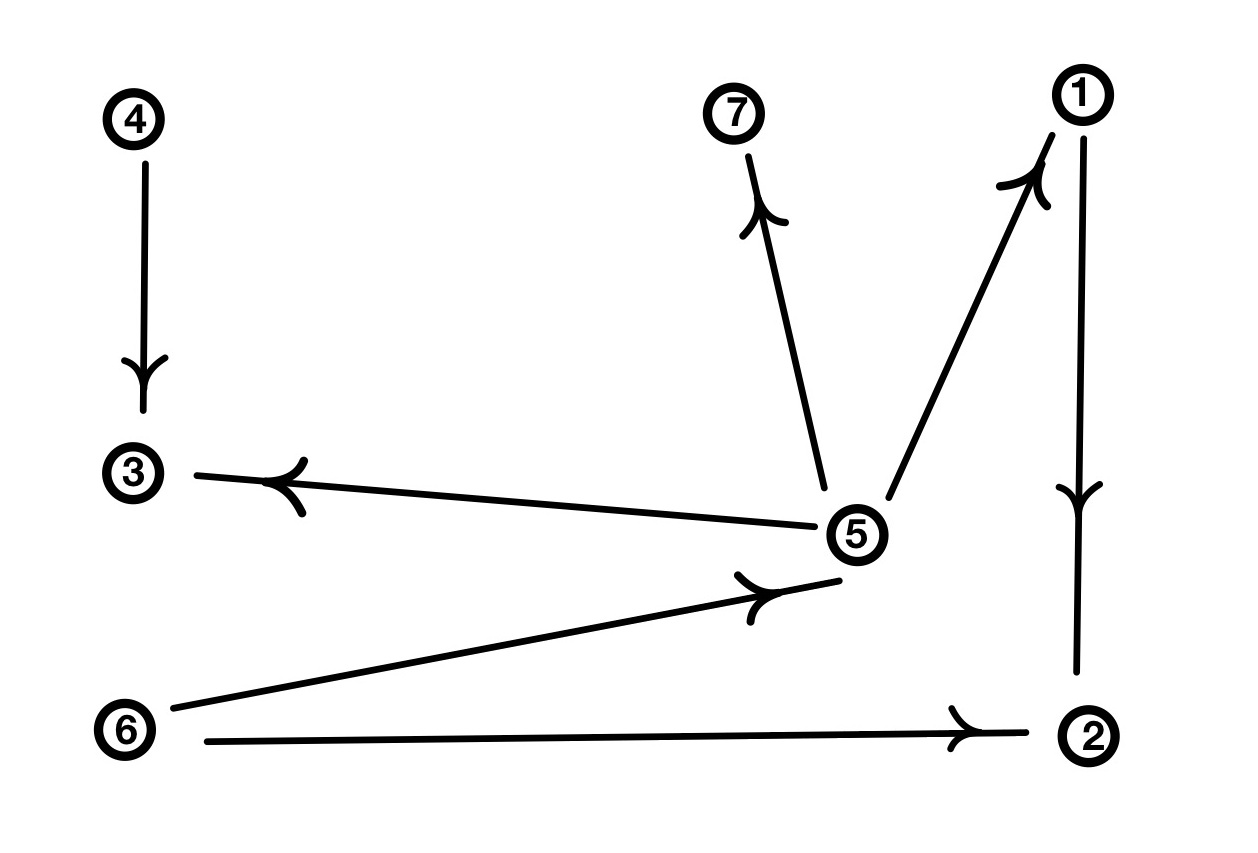
\includegraphics[width=0.6\textwidth]{recursos/capturas/CaminoCngrnt.jpg}
  \caption{Caminos $P=(1,2,6,5,7)$ y $Q=(4,3,5,1,2)$ congruentes.}
  \label{fig:CaminoCngrnt}
\end{figure}

En \cref{fig:CaminoCngrnt} se puede observar un par de camino congruentes $P=(1,2,6,5,7)$ y $Q=(4,3,5,1,2)$. Ahora introducimos una siguiente definición, dados un par de caminos congruentes $P$ y $Q$, decimos que $P$ evita a $Q$ si y solo si no hay flechas $(x_i,y_{i+1})$ en la misma orientación que las flechas $(x_i,x_{i+1})$. En el ejemplo anterior podemos afirmar que $P$ evita a $Q$, sin embargo, $Q$ no evita a $P$, ya que la flecha $(5,1)$ es derecha y la flecha $(5,5)$ al ser una flecha doble en particular es derecha y luego, $Q$ no evita a $P$.

\begin{figure}[H]
  \centering
  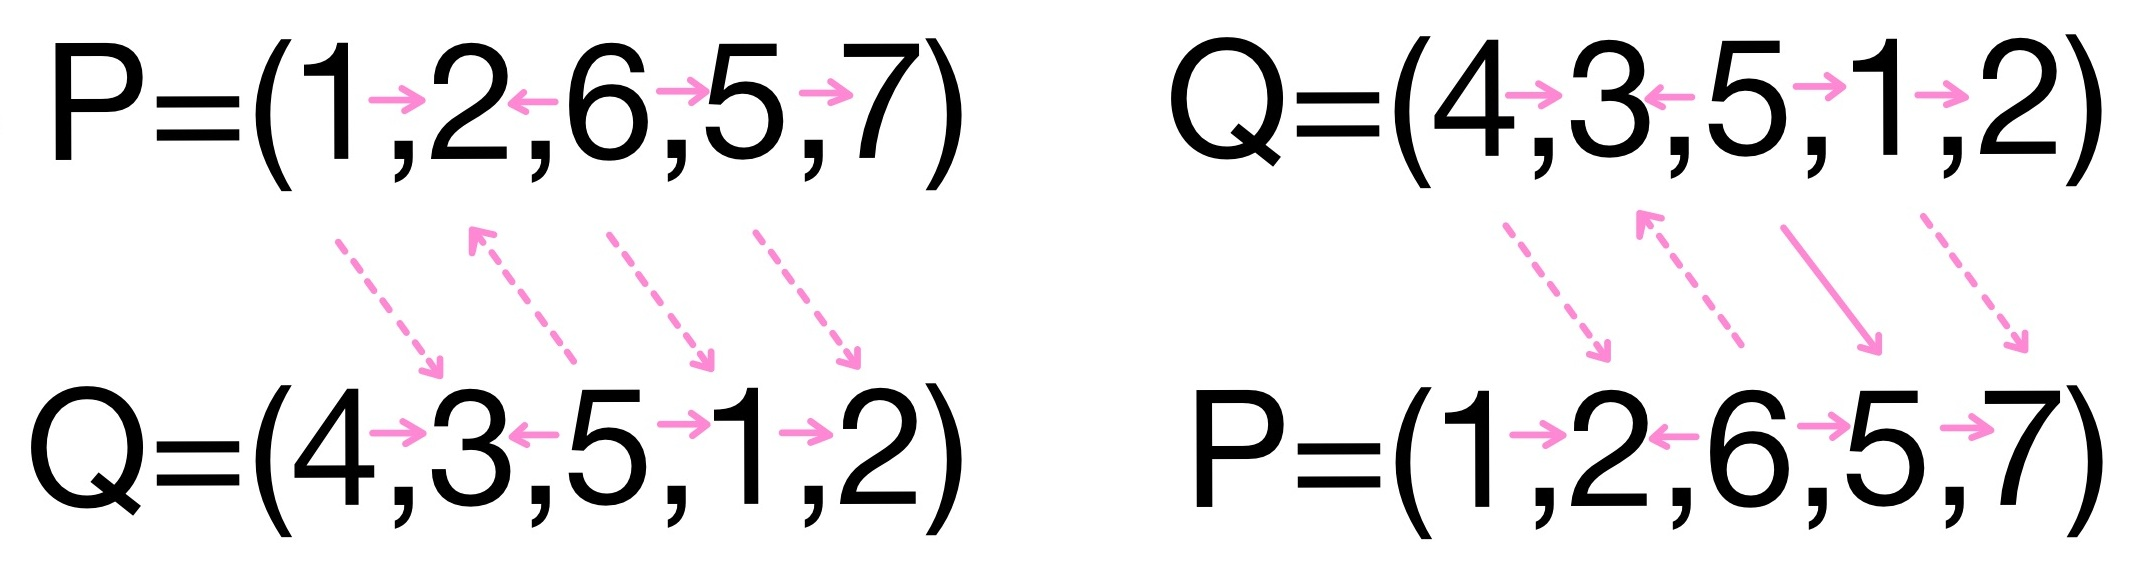
\includegraphics[width=0.5\textwidth]{recursos/capturas/Esqm.jpg}
  \caption{En este esquema las lineas punteadas son flechas que no pertenecen a $E(H)$, así a la izquierda se observa que $P$ evita a $Q$, a la derecha al se verifica que $Q$ no evita a $P$.}
  \label{fig:Esqm}
\end{figure}

Con todo lo anterior podemos dar paso a la definición de par invertible, estructura la cual nos permitirá caracterizar a las digráficas de intervalos ajustadas. Un par invertible en una digráfica $G$ es un par de vértices $u,v \in V(G)$ tales que cumplen, en primer lugar, que existen caminos congruentes $P$ de $u$ a $v$ y $Q$ de $v$ a $u$ de tal forma que $P$ evita a $Q$, y en segundo lugar, que existen caminos congruentes $P'$ de $v$ a $u$ y $Q'$ de $u$ a $v$, de tal forma que $P'$ evita a $Q'$.

A continuación damos un par de ejemplos de digráficas que tienen pares invertibles. Para nuestro primer ejemplo damos el $4$-ciclo $(1,2,3,4,1)$. Afirmamos que en esta digráfica los vértices $1$ y $3$ constituyen nuestro par invertible. Para esto damos los caminos congruentes $P=(1,2,3), Q=(3,4,1)$, notemos que así definidos los caminos son congruentes, tal y como se ilustra en el esquema de la derecha del $4$-ciclo de \cref{fig:InvrtblPair01} y además $P$ evita a $Q$ (las flechas en gris no existen en $F$). Recordando nuestra definición, necesitamos ahora otro par de caminos congruentes $P'$ y $Q'$, estos los definimos de la siguiente manera $P'=(3,2,1), Q'=(1,4,3)$ nuevamente usando el esquema de \cref{fig:InvrtblPair01}, se comprueba que dichos caminos son congruentes y que además $P'$ evita a $Q'$.

\begin{figure}[H]
  \centering
  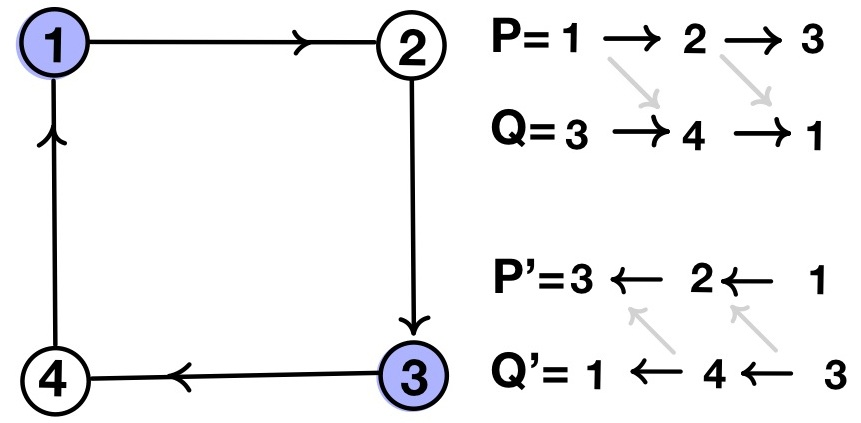
\includegraphics[width=0.5\textwidth]{recursos/capturas/InvtblPair01.jpg}
  \caption{Los vértices azules constituyen un par invertible. A la derecha los caminos congruentes $P,Q$, $P',Q'$.}
  \label{fig:InvrtblPair01}
\end{figure}

Un hecho interesante del ejemplo anterior es que es posible definir a $P'$ y a $Q'$ como los caminos inversos de $P$ y $Q$ respectivamente, donde entendemos que dado un camino $(x_0,x_1, \dots, x_n)$ el camino inverso es $(x_n,x_{n-1}, \dots, x_0)$. Aunque esto no se puede hacer en general, en este caso, la validez de lo anterior se debe a que tanto $P$ evita a $Q$ como $Q$ evita a $P$. 

A continuación hacemos simétricas las flechas de la gráfica anterior para tener un ejemplo donde es imposible definir a $P', Q'$ como los caminos inversos de $P, Q$ respectivamente. Veamos \cref{fig:InvrtblPair02}. Nuevamente tenemos que los vértices $1$ y $3$ son un par invertible. Algo importante a destacar es que los pares de caminos del ejemplo pasado, si bien siguen siendo congruentes, dejan de evitarse. Por ejemplo para que $P$ evite a $Q$ necesitamos que $(1,4),(2,1)\notin E(G)$, algo que no sucede en el presente ejemplo. Por lo anterior es necesario dar otro par de caminos $P$ y $Q$. Definimos $P=(1,2,2,3,3)$ y $Q=(3,3,4,4,1)$. Así definidos los caminos, son congruentes y además $P$ evita a $Q$. Si uno tratara de definir los caminos $P'$ y $Q'$ como los caminos inversos de $P$ y $Q$ respectivamente, uno caería en cuenta que así definidos el camino $P'$ no evita a $Q'$. Por lo que debemos encontrar otra forma alterna para definir a $P'$ y a $Q'$. Así, damos $P'=(3,4,4,1,1)$ y $Q'=(1,1,2,2,3)$ y definidos de esta forma, $P', Q'$ son caminos congruentes y son tales que $P'$ evita a $Q'$.

\begin{figure}[H]
  \centering
  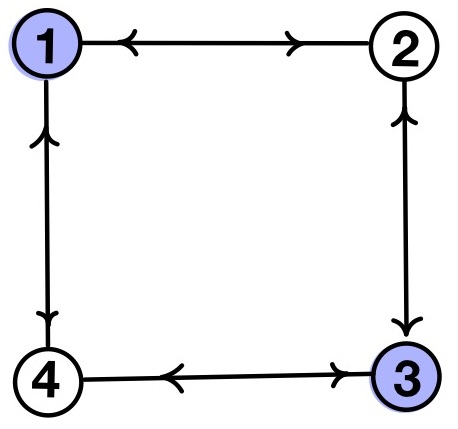
\includegraphics[width=0.3\textwidth]{recursos/capturas/InvrtblPair02.jpg}
  \caption{Los vértices azules constituyen un par invertible.}
  \label{fig:InvrtblPair02}
\end{figure}

Dada una digráfica $G$, definimos la digráfica de pares asociada a $G$, denotada por $G^{+}$ la cual está definida como $V(G^{+})=\{ (u,v)\in G\times G \colon\ u\neq v \}$ y diremos que $((u,v),(u',v'))\in F(G^{+})$ si y solo si sucede una de las siguientes dos cosas; $(u,u'),(v,v')\in E(G)$ y $(u,v')\notin E(G)$ o si sucede que $(u',u),(v',v)\in E(G)$ y $(v',u)\notin E(G)$. Usemos como ejemplo \cref{fig:InvrtblPair01} para dar la digráfica de pares asociada.

A partir del ejercicio anterior es fácil notar que la pareja de vértices $2,4$ también constituye un par invertible, algo igual de interesante es el hecho que pertenecen a la misma componente fuerte (flechas verdes). El siguiente teorema nos dice más sobre esta interesante observación.

\begin{teorema}
\label{teo:PairDigrph}
    Supongamos que $u$ y $v$ forman un par invertible de la digráfica $H$. Entonces $(u,v)$ y $(v,u)$ pertenecen a la misma componente fuertemente conexa $C$ de la digráfica de pares $H^+$. Más aún, cualquier otra pareja $(x,y)$ que pertenezca a $C$, cumple que su par revertido $(y,x)$ es también elemento de $C$.  Como consecuencia, si $(x,y) \in C$ entonces $x,y$ es un par invertible. Por otro lado si $H$ no tiene pares invertibles, entonces por cada componente fuerte $C$ de $H^+$, existe una componente fuerte $C' \neq C$ tal que $(x,y)\in C $ si y solo si $(y,x)\in C'$
\end{teorema}

\begin{proof}
    Probemos como primer punto que si $u,v$ son un par invertible, entonces $(u,v)$ y $(v,u)$ pertenecen a la misma componente fuertemente conexa.
    Ahora veamos que si $(x,y)\in C$ entonces $(y,x)\in C$. Para esto haremos una primera nota, $((u,v),(u',v'))\in E(H^+)$ implica que $((v',u'),(v,u))\in E(H^+)$, esto se puede corroborar observando la imagen 123123. Ahora sí, continuemos con la prueba, como $(x,y) \in C$ entonces la reversa de un camino cerrado que contiene a $(u,v),(x,y)$ es un camino cerrado que contiene a $(v,u),(y,x)$.    Luego, por concatenación de estos caminos cerrados, obtenemos otro camino cerrado que contiene a $(u,v),(v,u)$ y así podemos concluir que $(x,y),(y,x)$ pertenecen a la misma componente fuerte $C$.
    Finalmente si no existe un par invertible, para cada $(x,y)$ sabemos que $(y,x)$ no pertenece a la misma componente de $(x,y)$ pues en ese caso $x,y$ en efecto constituye un par invertible. Luego para cada $(x,y)\in C$ existe una componente $C'$ tal que $(y,x)\in C'$. 
\end{proof}

\begin{teorema}
\label{teo:OrdLnl}
    Sea $H$ una digráfica reflexiva, entonces un orden lineal $<$ es un ordenamiento m\'inimo si y solo si, para cualesquiera tres vértices $i<j<k$ tenemos que 
    $$ik\in E(H) \text{ implica } ij\in E(H)$$
    $$ki\in E(H) \text{ implica } ji\in E(H)$$
\end{teorema}
\begin{proof}
    Supongamos que $<$ es un ordenamiento m\'inimo, entonces $ab,jj\in E(H)$. Luego $\min(a,j) \min(b,j)\in E(H)$, donde $a,b \in \{ i,k\}$ con $a \neq b$.
    Ahora dado s $xy, x'y' \in E(H)$ veamos que $\min(x,x') \min(y,y')\in E(H)$. Todos los posibles casos son los siguientes:
    
    $ i) x<x' \wedge y<y' $ \hspace{1cm} $iii) x<x' \wedge y'<y $
    
    $ ii) x'<x \wedge y'<y $ \hspace{1cm} $iv) x'<x \wedge y<y' $

    De los dos primeros dos casos se concluye fácilmente que $\min(x,x') \min(y,y')\in E(H)$ pues:
    $$x<x' \wedge y<y' \Rightarrow \min(x,x') \min(y,y')=xy \text{ y } xy\in E(H) \text{por hipótesis.}$$
    $$x'<x \wedge y'<y \Rightarrow \min(x,x') \min(y,y')=x'y' \text{ y } x'y'\in E(H) \text{por hipótesis.}$$
    Los casos iii) y iv) hay que tratarlos de otra forma, probaremos solo iii) pues iv) es totalmente análogo.
    Tenemos que $x<x' \wedge y'<y\Rightarrow \min(x,x') \min(y,y')=xy' $ En este punto se nos presentan los siguientes casos; $x=y$ luego dado que $H$ es reflexiva, el lazo $xy\in E(H)$, el segundo caso $x<y' $. Como $y'<y$ obtenemos la cadena de desigualdades $x<y'<y$ y como $xy\in E(H)$ entonces $xy´\in E(H)$, como tercer y último caso, tenemso que $y'<x$. Entonces $x<x'$ así $y'<x<x'$ y $x'y'\in E(H)$ luego $xy'\in E(H)$. En cualquiera de los dos casos anteriores se tiene que $min(x,x')min(y,y')\in E(H)$. Por lo que podemos concluir que en efecto $<$ es un ordenamiento mínimo.
\end{proof}

A partir del teorema anterior podemos obtener el siguiente corolario.
\begin{corolario}
    Sea $H$ una dgráfica reflexiva. Un ordenamieno lineal de los vértices de $H$ es un ordenamiento mínimo si y solo si para cada vértice $v$, los vértices que siguen a $v$ en el orden, consisten de: i) Primero aparecen (en el orden) los vértices que son adyacentes a $v$ por flechas simétricas. ii) En segundo lugar aparecen los vértices que son adyacentes a v por aristas asimétricas, además son todas derechas o todas izquierdas, iii) Finalmente tenemos vértices que no tinen flechas desde o hacia $v$
\end{corolario}

\begin{proof}
    Esto es fácil de verificar, supongamos que $u<v<w$ y supongamos que $uw,wu\in E(H)$ veremos que si esto pasa por fuerza $v$ debe tener también flechas dobles hacia $u$, es decir, no puede tener flechas asimétricas ni puede no tener flechas desde o hacia $u$.
    Por la primera consecuencia de \cref{teo:OrdLnl} se tiene que $uv\in E(H)$, y por la segunda consecuencia, tenemos que $vu\in E(H)$. Así $v$ debe tener flechas simétricas hacia $u$. 
    Verifiquemos rápidamente que si $u<v<w$ y hay una flecha asimétrica de $u$ a $w$, entonces debe haber una flecha asimétrica con la misma dirección de $u$ a $v$. Nuevamente el resultado es bastante inmediato del \cref{teo:OrdLnl}, ya que si $uw\in E(H)$ entonces $uv\in E(H)$ o análogamente si $wu\in E(H)$ entonces $vu\in E(H)$.
\end{proof}

\begin{teorema}
    Una digráfica reflexiva es una digráfica de intervalos ajustada si y solo si admite un ordenamiento mínimo.
\end{teorema}

\begin{proof}
    Dado un ordenamiento mínimo de una digráfica reflexiva $H$, podemos ordenar los puntos iniciales de $I_v$ y de $J_v$ en el mismo orden en los cuales aparecen los vértices $v\in V(H)$ respecto al ordenamiento mínimo y definimos los intervalos $I_v$ y $J_v$ como:
\end{proof}
A continuación vemos un ejemplo mas de una digráfica de intervalos ajustada